\documentclass{article}

\usepackage[final]{neurips_cerri_2022}

\usepackage[utf8]{inputenc} % allow utf-8 input
\usepackage[T1]{fontenc}    % use 8-bit T1 fonts
\usepackage{hyperref}       % hyperlinks
% \hypersetup{
%     colorlinks=true,
%     linkcolor=blue,}
\usepackage{url}            % simple URL typesetting
\usepackage{booktabs}       % professional-quality tables
\usepackage{amsfonts}       % blackboard math symbols
%\usepackage{amsmath}
% \usepackage{amssymb,amsmath,color}
\usepackage{nicefrac}       % compact symbols for 1/2, etc.
\usepackage{microtype}      % microtypography
\usepackage{xcolor}         % colors
\usepackage{algorithm}
\usepackage{algpseudocode}
\usepackage{subfigure}
\usepackage{graphicx}
\graphicspath{ {./media/} }

%%symbols declaration 
% \DeclareMathAlphabet\mathbfcal{OMS}{cmsy}{b}{n} %for calligraphy letters
% \DeclareMathOperator*{\argmin}{argmin}
% \DeclarePairedDelimiter{\norm}{\lVert}{\rVert} 
%end symbol declaration


%%%%%%%%%%%%%%%%%%%%%%%%%%%%%%%%%%%%%%%%%%%%%%%%%%%%%%%%%%%%%%%%%%%%%%%%%%%%%
%%%%%%%%%%%%%%%%%%%%%%%%%%%%%%%%%%%%%%%%%%%%%%%%%%%%%%%%%%%%%%%%%%%%%%%%%%%%%


\title{REAL TIME SYSTEMS ASSIGNMENT: SCHEDULING FOR AN AUTONOMOUS \newline ROBOT NAVIGATION ALGORITHM\newline\newline30 SEPTEMBER 2022 }

\author{
  Francesco Cerri\\
  \texttt{francesco.cerri2@studio.unibo.it} \\
  \hyperlink{github.com/gnoccoalpesto}{github.com/gnoccoalpesto}
}


%%%%%%%%%%%%%%%%%%%%%%%%%%%%%%%%%%%%%%%%%%%%%%%%%%%%%%%%%%%%%%%%%%%%%%%%%%%%%
%%%%%%%%%%%%%%%%%%%%%%%%%%%%%%%%%%%%%%%%%%%%%%%%%%%%%%%%%%%%%%%%%%%%%%%%%%%%%
\begin{document}




\maketitle


%%%%%%%%%%%%%%%%%%%%%%%%%%%%%%%%%%%%%%%%%%%%%%%%%%%%%%%%%%%%%%%%%%%%%%%%%%%%%%


\section{Introduction to the problem}               \label{intro}

I decided to present a system where a navigation stack for a mobile robot is scheduled. The system presents 4 tasks: highest priority one's purpose is to verify the consistency of the system, whilst others' is to properly let the robot sense the environment and move inside of it.

\subsection{Task set}                               \label{tasks}

Task set is composed by:

\begin{enumerate}
    \item \textbf{tMonitor task} ($\tau_{M}$): is responsable to checks if all other tasks are correctly operating, respawning them if needed. Has maximum priority to ensure the safety of the system, phased activation since it must wait for other tasks to start, low computation time due to its ping-like behaviour, high period and does not use any resource;
    
    \item \textbf{tCamera task} ($\tau_{V}$):  acquires the video from the hardware sensor and publishes it, after preprocessing (for example identifying the AR markers usefull to locate the bodies in the field of view). Has high priority since it's the source of vision for downstream nodes, medium computation time to simulate the presence of a dedicated hardware in the system (i.e. a GPU), medium period and uses (by publishing it) the \textbf{Image resource};
    
    \item \textbf{tCollision task} ($\tau_{C}$): uses processed camera stream to reconstruct the physical objects in the environment. Has lower priority, high computational time, and uses both camera as well as \textbf{Objects resource}, the first as input, while it publishes the latter;
    
    \item \textbf{tPlanner task} ($\tau_{P}$): plans robot path using identified objects. Has the lowest priority since its the final user, very long computational time and period and uses as input object resource.
\end{enumerate}

All tasks are \textbf{periodic} and have \textbf{fixed priority}, with:

\begin{center}
    \emph{$P(\tau_{M}) > P(\tau_{V})> P(\tau_{C})> P(\tau_{P})$}
\end{center}    
\medskip{}

\subsection{Resources and constraints}              \label{resources}

Two resources are available in the system:

\begin{enumerate}
    \item Image resource ($R_{I}$): the visual data coming from $\tau_{V}$, used by $\tau_{C}$;
    \item Objects resource ($R_{O}$): the collision coming from $\tau_{C}$, used by $\tau_{P}$.
\end{enumerate}

Both resources have a \textbf{single instance}. Scheduling must be done considering that when $\tau_{C}$ is using the R$_{I}$ resource, $\tau_{V}$ must not update it to avoid inconsistency in the data; the same thing must happen for $\tau_{P}$, R$_{O}$ and $\tau_{C}$ respectively. Moreover, \textbf{resources are nested} for the same reason.

\begin{table}[H]                                    \label{tab_ceilings}
  \centering
  \begin{tabular}{ll}
     Resource &   $C(R_{k})$\\
     \midrule
    $R_{I}$ &       $P(\tau_{V})$    \\
    $R_{O}$ &       $P(\tau_{C})$    \\
    \bottomrule
  \end{tabular}
  \medskip{}
  \caption{Resource ceilings based on priorities}
  \medskip{}
\end{table}

\subsection{Implementation}                           \label{code}

Simulation of the system is performed using VxWorks7, setting as \textbf{clock frequency 20 Hz}.
\footnote{Namely, every unit of time represented lasts 50 ms.}
\footnote{This avoids heavy interference by the Windows host system.}\newline
Task set $\Gamma$ presents the following parameters:

\begin{table}[H]                                    \label{tab_set}
  \centering
  \begin{tabular}{lllllllll}
    $\Gamma$ &   $\Phi_{i}$ & $C_{i}$ & $T_{i}$ & $U_{i}$ & $t_{i}^{I}$ & $\delta_{i}^{I}$ & $t_{O}$ & $\delta_{i}^{O}$\\
    \cmidrule(r){2-5}
    \cmidrule(r){6-7}
    \cmidrule(r){8-9}
    $\tau_{M}$ & 20  &  2 &         16 &    .125 &     &       &           &           \\
    $\tau_{V}$ & 0   &  6 &         30 &    .2 &     .5 &   5.5 &            &      \\
    $\tau_{C}$ & 0   &  10 &        40 &    .25 &     .5 &   9.5  &          3 &      7\\
    $\tau_{P}$ & 0   &  16 &        60 &    .2667 &       &       &          .5 &     7\\
    \bottomrule
  \end{tabular}
  \medskip{}
  \caption{Task Set}
  \medskip{}
\end{table}

with an \textbf{hyperperiod}H=240 and \textbf{harmonic task groups} of periods 16,\{30,60\},40.


%%%%%%%%%%%%%%%%%%%%%%%%%%%%%%%%%%%%%%%%%%%%%%%%%%%%%%%%


\section{Analysis}                      \label{analysis}

Required conditon of \textbf{Processor Utilization Criterion} is satisfied being:

\begin{center}
 $\sum_i \nicefrac{C_{i}}{T_{i}} = .125 + .2 + .25 + .2667 = 0.8417 < 1$
\end{center}

Since all tasks are periodic, analysis will be performed starting from \textbf{Liu-Layland utilization bounds}(LL), switching to \textbf{Hyperbolic Bounds}(HB) in case of failure and \textbf{Response Time Analysis} (RTA) in last instance.

\subsection{Blocking times with different Resource Access Protocols}    \label{blocking}

\begin{table}[H]
  \label{network_table}
  \centering
  \begin{tabular}{llll}
    $\Gamma$ &    $B_{i}^{NPP}$ & $B_{i}^{HLP}$  & $B_{i}^{PIP}$\\
    \midrule
    $\tau_{M}$ &    9.5  &      0   &           16.5 \\
    $\tau_{V}$ &    9.5 &       9.5 &           9.5\\
    $\tau_{C}$ &    7 &         7 &             7\\
    $\tau_{P}$ &    0 &         0 &             0\\
    \bottomrule
  \end{tabular}
  \medskip{}
  \caption{Blocking time under different Resource Access Protocols}
\end{table}

Computation is performed considering no prehemption for NPP, ceilings for HLP, and (possible) chained blocking for PIP.

\subsection{Bounds and Response Time Analysis for task set}

Considering that

\begin{itemize}
    \item $B_{V}^{NPP} == B_{V}^{HLP} == B_{V}^{PIP}$
    \item $B_{C}^{NPP} == B_{C}^{HLP} == B_{C}^{PIP}$
    \item $B_{P}^{NPP} == B_{P}^{HLP}== B_{\tau_{P}}^{PIP}$
\end{itemize}

we can use \textbf{extended analysis} to confirm feasibility of the task set:

\begin{center}                          \label{llb}
    \medskip{}
    $\tau_{M}^{NPP} : U_{M} + B_{M}^{NPP} = .125 + .5937 = .718 < LL_{1} =1$\\\medskip{}
    $\tau_{M}^{HLP} : U_{M} + B_{M}^{HLP} = .125 + 0 = .125 < LL_{1} =1$\\\medskip{}
    $\tau_{M}^{PIP} : U_{M} + B_{M}^{PIP} = .125 + 1.031 = 1.156 > LL_{1} =1$\\\medskip{}
    $\tau_{V}^{NPP} : U_{M} + U_{V} + B_{V}^{NPP} = .125+ .2+ .3167 = .6417 < LL_{2} =.828$\\\medskip{}
    $\tau_{C}^{NPP} : U_{M} + U_{V} + U_{C} + B_{C}^{NPP} = .125 + .2 + .25 + .175 = .75< LL_{3} =.779$\\\medskip{}
    $\tau_{P}^{NPP} : U_{M} + U_{V} + U_{C} + U_{P} + B_{P}^{NPP} = .125+.2+.25+.2667 = .8416 > LL_{3} =.779$\\\medskip{}
\end{center}
\textbf{Using bounds, theoretical feasibility of PIP under fixed priorities is automatically not provable}, yet can still be searched for any other protocol. Let's use HB on $\tau_{P}$:

\begin{center}                      \label{hb}
    $(1+U_{M})\cdot(1+ U_{V})\cdot(1+ U_{O})\cdot (1+ U_{P} + B_{P}^{NPP}) = 1.125\cdot1.2\cdot1.25 \cdot1.267 =2.138> 2$
\end{center}

Still feasibility is yet to be proven. RTA is the last (simple) possibility for $\tau_{P}$:

\begin{center}                      \label{rta}
    $R_{P}^{0}= \sum_{i}C_{k} + B_{P}^{NPP}=2+6+10+16=34<T_{P}=60$\\\medskip{}
    $R_{P}^{1}= \sum_{j}\left \lceil{\nicefrac{R_{P}^{0}}{T_{j} }}\right \rceil *C_{j} + C_{P} + B_{P}^{NPP}=16+6+12+10 =44<60$\\\medskip{}
    $R_{P}^{2}= 16+6+12+20=54<60$\\\medskip{}
    $R_{P}^{3}=R_{P}= 16+8+12+20=56<60$\\\medskip{}
\end{center}

\textbf{proving theoretical feasibility under fixed priorities for NPP and HLP}.


%%%%%%%%%%%%%%%%%%%%%%%%%%%%%%%%%%%%%%%%%%%%%%%%%%%%%%%%%%%%%%%%%%%%%%%%%%%%


\section{Simulation and results}                   \label{simulation}

Using VxWorks I initially show a feasible schedule under \textbf{no resource access protocol}. Displayed results are taken from VxW's \textbf{System Viewer} tool.

\begin{figure}[H]                                   \label{fig_nop}
  \centering
  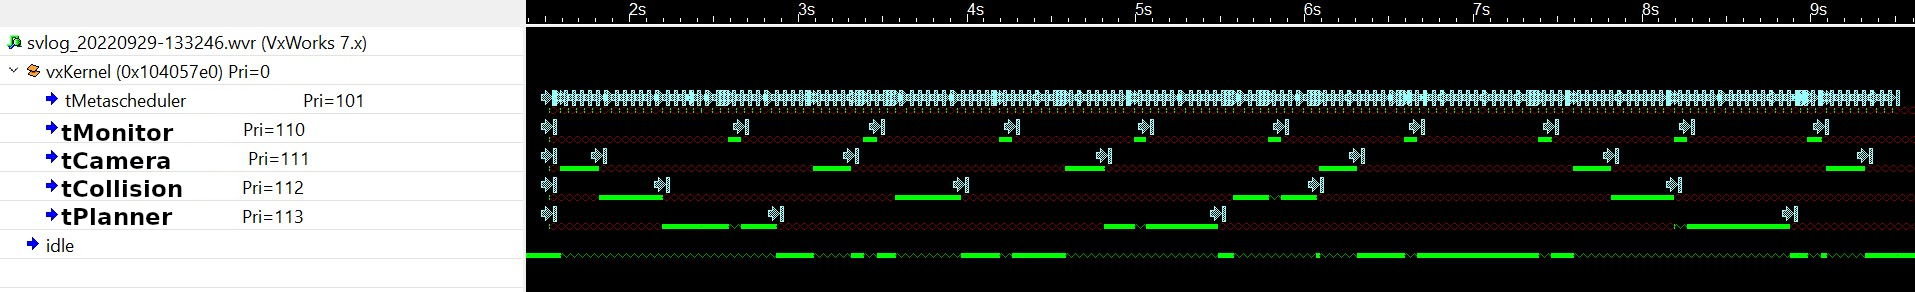
\includegraphics[width=13.9cm]{media/nop_phased.jpg}
  \caption{$\Gamma$ under No Protocol and phased activation.}
\end{figure}

It appears clear that \textbf{no tasks register an overrun}, yet response time are pretty long
\begin{itemize}
    \item \begin{center}
            NOP: R$_{P}=2$, R$_{V}=7$, R$_{C}=15$, R$_{P}=29$
        \end{center}
\end{itemize}

suggest the need for a Resource Access Protocol.

\subsection{Simulation for R.A.P.s}                 \label{rap}

Here, only simulations for \textbf{Non Prehemptive Protocol} (NPP),\textbf{Highest Locker Protocol} (HLP) and \textbf{Priority Inheritance Protocol}, with \textbf{phased activations} are showed.\vspace{.3cm}\\
Since it is possible to find a feasible schedule, \textbf{feasibilty of PIP under fixed priorities is proven}.

\begin{figure}[H]                                       \label{fig_rap}
    \subfigure[]{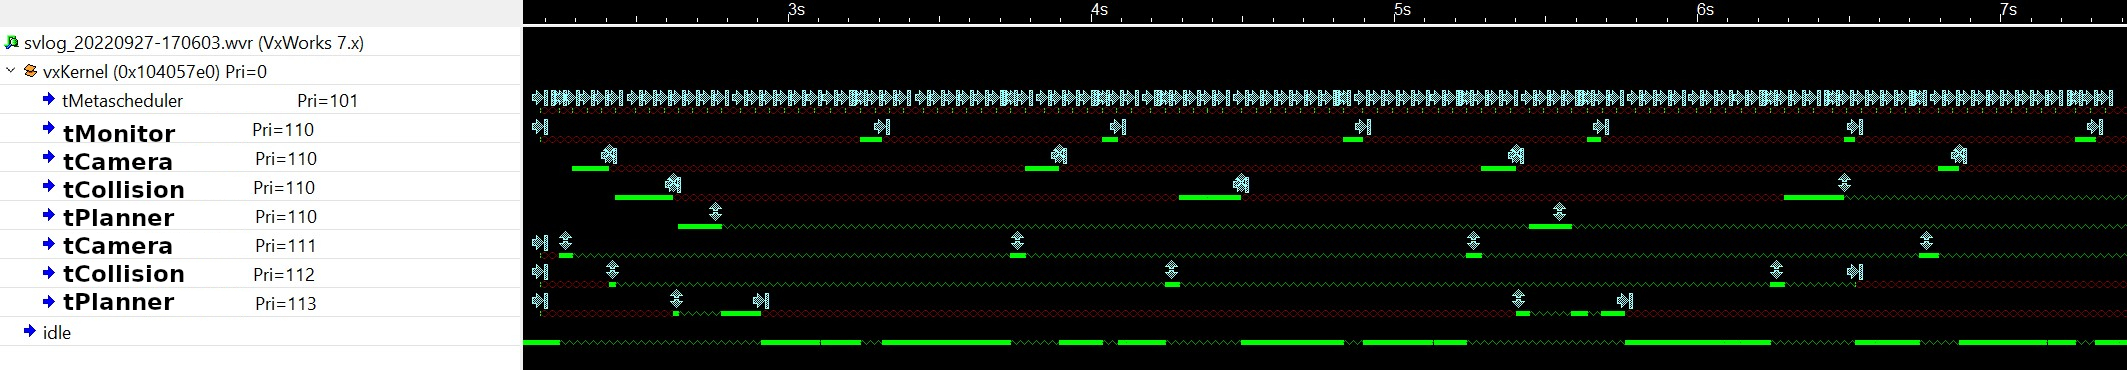
\includegraphics[width=13.9cm]{media/npp_phased.jpg}}
    \subfigure[]{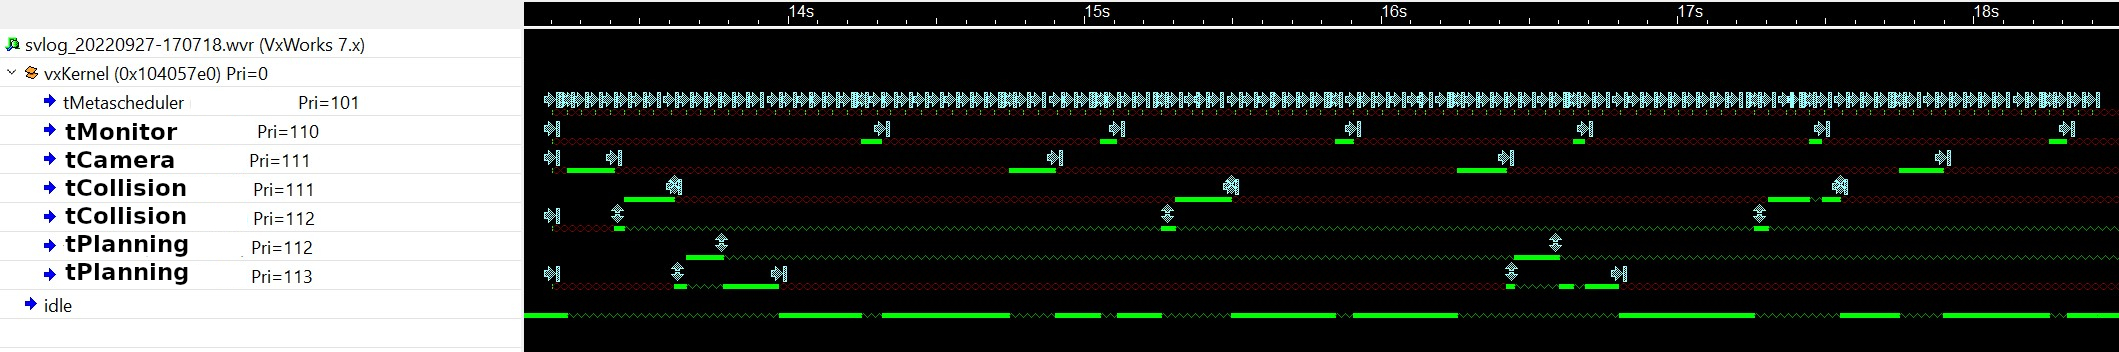
\includegraphics[width=13.9cm]{media/hlp_phased.jpg}}
    \subfigure[]{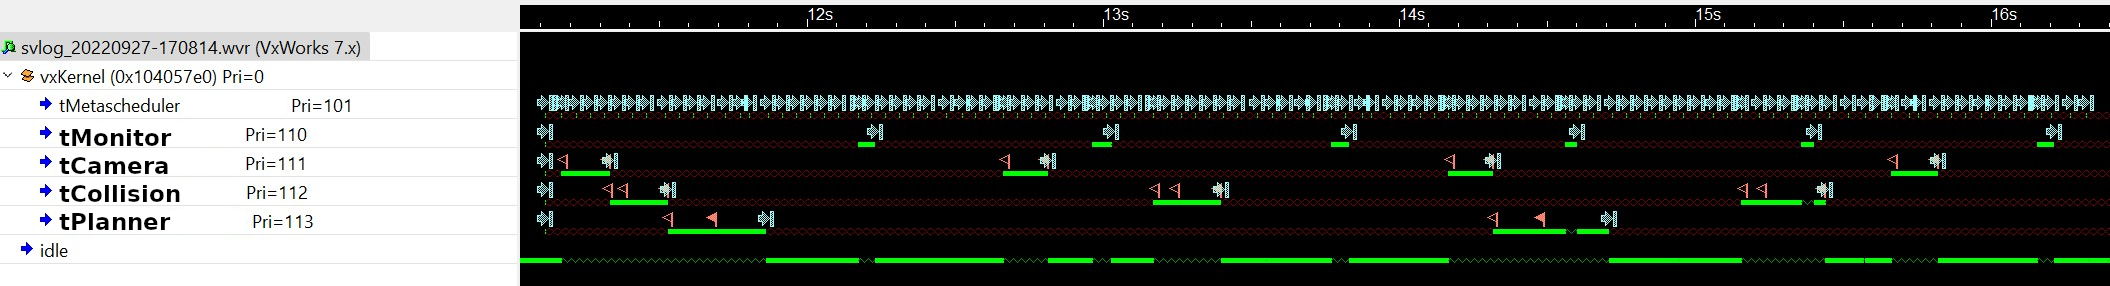
\includegraphics[width=13.9cm,height=2.6cm]{media/pip_phased.jpg}}
    \caption{Simulations for phased activations of: (a) NPP, (b) HLP, and (c) PIP protocols}
\end{figure}

Even in this case \textbf{no tasks presents overruns}, yet response times are consistently lower:

\begin{itemize}
    \item \begin{center}
            NPP$^{Ph}$: R$_{P}=4$, R$_{V}=5$, R$_{C}=9$, R$_{P}=16$
        \end{center}
    \item \begin{center}
            HLP$^{Ph}$: R$_{P}=2$, R$_{V}=5$, R$_{C}=9$, R$_{P}=16$
        \end{center}
    \item \begin{center}
            PIP$^{Ph}$: R$_{P}=2$, R$_{V}=5$, R$_{C}=9$, R$_{P}=15$
        \end{center}
\end{itemize}

For completeness, I also tested \textbf{non-phased activations}, resulting in \textbf{no overruns} and the following response times:

\begin{itemize}
    \item \begin{center}
            NPP$^{N-Ph}$: R$_{P}=2$, R$_{V}=4$, R$_{C}=8$, R$_{P}=15$
        \end{center}
    \item \begin{center}
            HLP$^{N-Ph}$: R$_{P}=2$, R$_{V}=4$, R$_{C}=8$, R$_{P}=15$
        \end{center}
    \item \begin{center}
            PIP$^{N-Ph}$: R$_{P}=2$, R$_{V}=4$, R$_{C}=8$, R$_{P}=15$
        \end{center}
\end{itemize}

\subsection{Conclusions}                                \label{conclusions}

For what it concerns performances, apart from Phased NPP, all protocol show a small and constant response time for the highest priority tMonitor. Non phased activations also show a smaller response time for all tasks.

Besides that, all R.A.P. behaves very similarly, hence the more logical choice would be selecting the easier one to implement.\\


\subsection{Future work}                                \label{future}

An interesting evolution for this project would be implementing a third resource representing the bandwidth of the communication channel between nodes as a  \textbf{multi-instance} resource. Other resource will be nested inside of it, to represent the necessity of using the network every time a tasks needs to receive of send data. A possible implementation would be

\begin{table}[H]                                    \label{tab_net}
  \centering
  \begin{tabular}{lll}
    $\Gamma$ &  $t_{B}$ & $\delta_{i}^{B}$\\
    \cmidrule(r){2-3}
    $\tau_{M}$ & .5 &  1.5\\
    $\tau_{V}$ & .5   & 5.5\\
    $\tau_{C}$ & .5   &  9.5\\
    $\tau_{P}$ & .5   &  7\\
    \bottomrule
  \end{tabular}
  \medskip{}
  \caption{Tasks' bandwidth utilization.}
  \medskip{}
\end{table}


%%%%%%%%%%%%%%%%%%%%%%%%%%%%%%%%%%%%%%%%%%%%%%%%%%%%%%%%%%%%%%%%%%%%%%%%%%%%%%


\vspace{2cm}
\section*{References}                               \label{ref}

\medskip

{
[1] Buttazzo, G \ (2011) Hard Real-Time Computing Systems. Springler.\\ \url{https://doi.org/10.1007/978-1-4614-0676-1}

[2] Torroni, G \ (2021) Lectures of the course "Real Time Systems for Automation, M". Università di Bologna.\\ \url{https://www.unibo.it/en/teaching/course-unit-catalogue/course-unit/2021/402384}
}


%%%%%%%%%%%%%%%%%%%%%%%%%%%%%%%%%%%%%%%%%%%%%%%%%%%%%%%%%%%%%


\appendix

\vspace{2cm}
\section{Code and definitions}                      \label{code}

For the code and documentation, please refer to\\ \url{https://github.com/gnoccoalpesto/vx_rover}




\end{document}
%%%%%%%%%%%%%%%%%%%%%%%%%%%%%%%%%%%%%%%%%%%%%%%%%%%%%%%%%%%%%
%%%%%%%%%%%%%%%%%%%%%%%%%%%%%%%%%%%%%%%%%%%%%%%%%%%%%%%%%%%%%
